%!TEX root = curso_EDA_SLIDES.tex

\section{O Curso}
\begin{frame}


\frametitle{Disciplina}

\begin{block}{Estrutura de Dados -- EDA001}

\begin{itemize}
\item \emph{\textbf{Turma:}} 
\item \emph{\textbf{Professor:}} Claudio Cesar de Sá
  \begin{itemize}
  \item \texttt{claudio.sa@udesc.br}
  \item Sala 13 Bloco F
  \end{itemize}
\item \emph{\textbf{Carga horária:}} 72 horas-aula 
\textcolor{red}{$\bullet$}~Teóricas: 36 \textcolor{red}{$\bullet$}~Práticas: 36
\item \emph{\textbf{Curso:}} BCC
\item \emph{\textbf{Requisitos:}} LPG, Linux, LMA, conhecimento da linguagem C
\item \emph{\textbf{Período:}} 2º semestre de 2017
\item \emph{\textbf{Horários:}}
  \begin{itemize}
  \item 3ª 15h20 (2 aulas) - F-205  -- aula expositiva
  \item 5ª 15h20 (2 aulas) - F-205 -- lab
  
  \end{itemize}

\end{itemize}

\end{block}

\end{frame}


%-------------------------------------
\begin{frame}
\frametitle{Ementa}

\begin{block}{Ementa}
Representação e manipulação de tipos abstratos de dados. Estruturas lineares. Introdução a estruturas hierárquicas. Métodos de classificação. Análise de eficiência. Aplicações.
\end{block}

\end{frame}

%-------------------------------------
\begin{frame} [allowframebreaks=0.9]
\frametitle{Objetivos}

\begin{itemize}
\item \emph{\textbf{Geral:}} 
 
 \textcolor{red}{FALTANDO}

\newpage
\item \emph{\textbf{Específicos:}} 

  \begin{itemize}
  \item  \textcolor{red}{FALTANDO}
  \item  
  
  \end{itemize}

\end{itemize}

\end{frame}

%-----------------------------------------------------------------------

\begin{frame}
\frametitle{Livros que estarei usando ...}

\begin{columns}
\begin{column}{.5\textwidth}
\centering
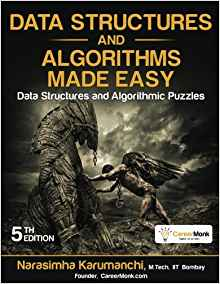
\includegraphics[height=6cm, width=5cm]{figs/fig_gerais/capa_livro_made_easy.jpeg}

\end{column}

\begin{column}{.5\textwidth}
\centering

\includegraphics[height=6cm, width=5cm]{figs/fig_gerais/capa_livro_program_design_C.jpeg}

\end{column}

\end{columns}


\end{frame}
%-----------------------------------------------------------------------

\begin{frame}
\frametitle{Conteúdo programático}

    \begin{itemize}
      \item  \textcolor{red}{FALTANDO}
      
    \end{itemize}
    
\end{frame}


%-----------------------------------------------------------------------
\begin{frame}
\frametitle{Bibliografia UDESC}

    \begin{itemize}
     
      \item  \textcolor{red}{FALTANDO}
      
    \end{itemize}
    
\end{frame}

%-----------------------------------------------

\begin{frame}
\frametitle{Conteúdo programático}


    \begin{itemize}
      \item  \textcolor{red}{FALTANDO}
      
    \end{itemize}
\end{frame}
---------------------------

\subsection{Ferramentas}
\begin{frame}

    \frametitle{Ferramentas}

    \begin{itemize}
      \item Linguagem C
      \item Codeblock
      \item Linux
      % \url{http://ccl.northwestern.edu/netlogo/docs/} (escondido in WEB)
      
    \end{itemize}
\end{frame}

%%%%%%%%%%%%%%%%%%%%%%%%%%%%%%%%%%%%%%%%%%%%%%%%%%%%%%%%%%%%%%%%%%%%%

\subsection{Metodologia e avaliação}  

\begin{frame}[allowframebreaks=0.9]

\frametitle{Metodologia e avaliação}

\textbf{Metodologia:} \\

\textit{As aulas serão expositivas e práticas. A cada novo assunto tratado, exemplos 
 são demonstrados utilizando ferramentas computacionais adequadas para consolidar os conceitos 
 tratados. 
 }


\newpage
    \textbf{Avaliação}

    \begin{itemize}
    \item Tres provas -- $\approx$  90\%\\
      
	\quad \textcolor{red}{$\bullet$}~$P_1$: xx/set\\
	\quad \textcolor{red}{$\bullet$}~$P_2$: yy/out\\
	\quad \textcolor{red}{$\bullet$}~$P_2$: zz/nov\\(provão: todo conteúdo)


      \item Exercícios de laboratório  -- $\approx$ \%
      
     %  \item O artigo (resultados da implementação)  -- $\approx$ 30\%

%      \item Para o artigo: muito material será fornecido em \LaTeX ...

 %     \item Apresentação de um artigo estudado sobre SMA -- $\approx$ 15\%
 
      \item Presença e participação
      
      \item Média para aprovação: 6,0 (seis)\\
      Nota maior ou igual a 6,0, repito a mesma no Exame Final. Caso contrário, regras da UDESC
      
    \end{itemize}

\end{frame}



\subsection{Dinâmica}
\begin{frame}

    \frametitle{Dinâmica de Aula}

    \begin{itemize}
      
      \item Teoria na 3a. feira
      \item Prática na 5a. feira
      \item E/ou 50\% do tempo em teoria, 50\% implementações 
      
    \end{itemize}
\end{frame}



%%%%%%%%%%%%%%%%%%%%%%%%%%%%%%%%%%%%%%%%%%%%%%%%%%%%%%%%%%%%%%%%%%%%%

\subsection{Referências}  
%[allowframebreaks=0.9]

%-------------------------------------
\begin{frame}[allowframebreaks=0.9]
\frametitle{Bibliografia}  

\textbf{Básica:} 
\begin{itemize}

\item  \textcolor{red}{FALTANDO}
\item  \textcolor{red}{FALTANDO}
\item  \textcolor{red}{FALTANDO}
\item  \textcolor{red}{FALTANDO}
\item  \textcolor{red}{FALTANDO}

\item \url{https://github.com/claudiosa/CCS/tree/master/estrutura_dados_EDA}

\end{itemize}

\textbf{Complementar:}

\begin{itemize}
\item  \textcolor{red}{FALTANDO}
\item  \textcolor{red}{FALTANDO}
\item  \textcolor{red}{FALTANDO}
\end{itemize}

\end{frame}




%%%%%%%%%%%%%%%%%%%%%%%%%%%%%%%%%%%%%%%%%%%%%%%%%%%%%%%%%%%%%%%%%%%%%
